\documentclass[tikz,border=18pt]{standalone}
\usepackage[utf8]{inputenc}
\usepackage[T1]{fontenc}
\usepackage{amsmath,amssymb}
\usepackage{tikz}
\usetikzlibrary{positioning,arrows.meta,fit,backgrounds,shadows,calc}

\definecolor{ehrblue}{RGB}{30, 64, 175}
\definecolor{iotgreen}{RGB}{5, 150, 105}
\definecolor{corepurple}{RGB}{109, 40, 217}
\definecolor{amberalert}{RGB}{217, 119, 6}
\definecolor{slateborder}{RGB}{100, 116, 139}
\definecolor{darkslate}{RGB}{30, 41, 59}

\begin{document}
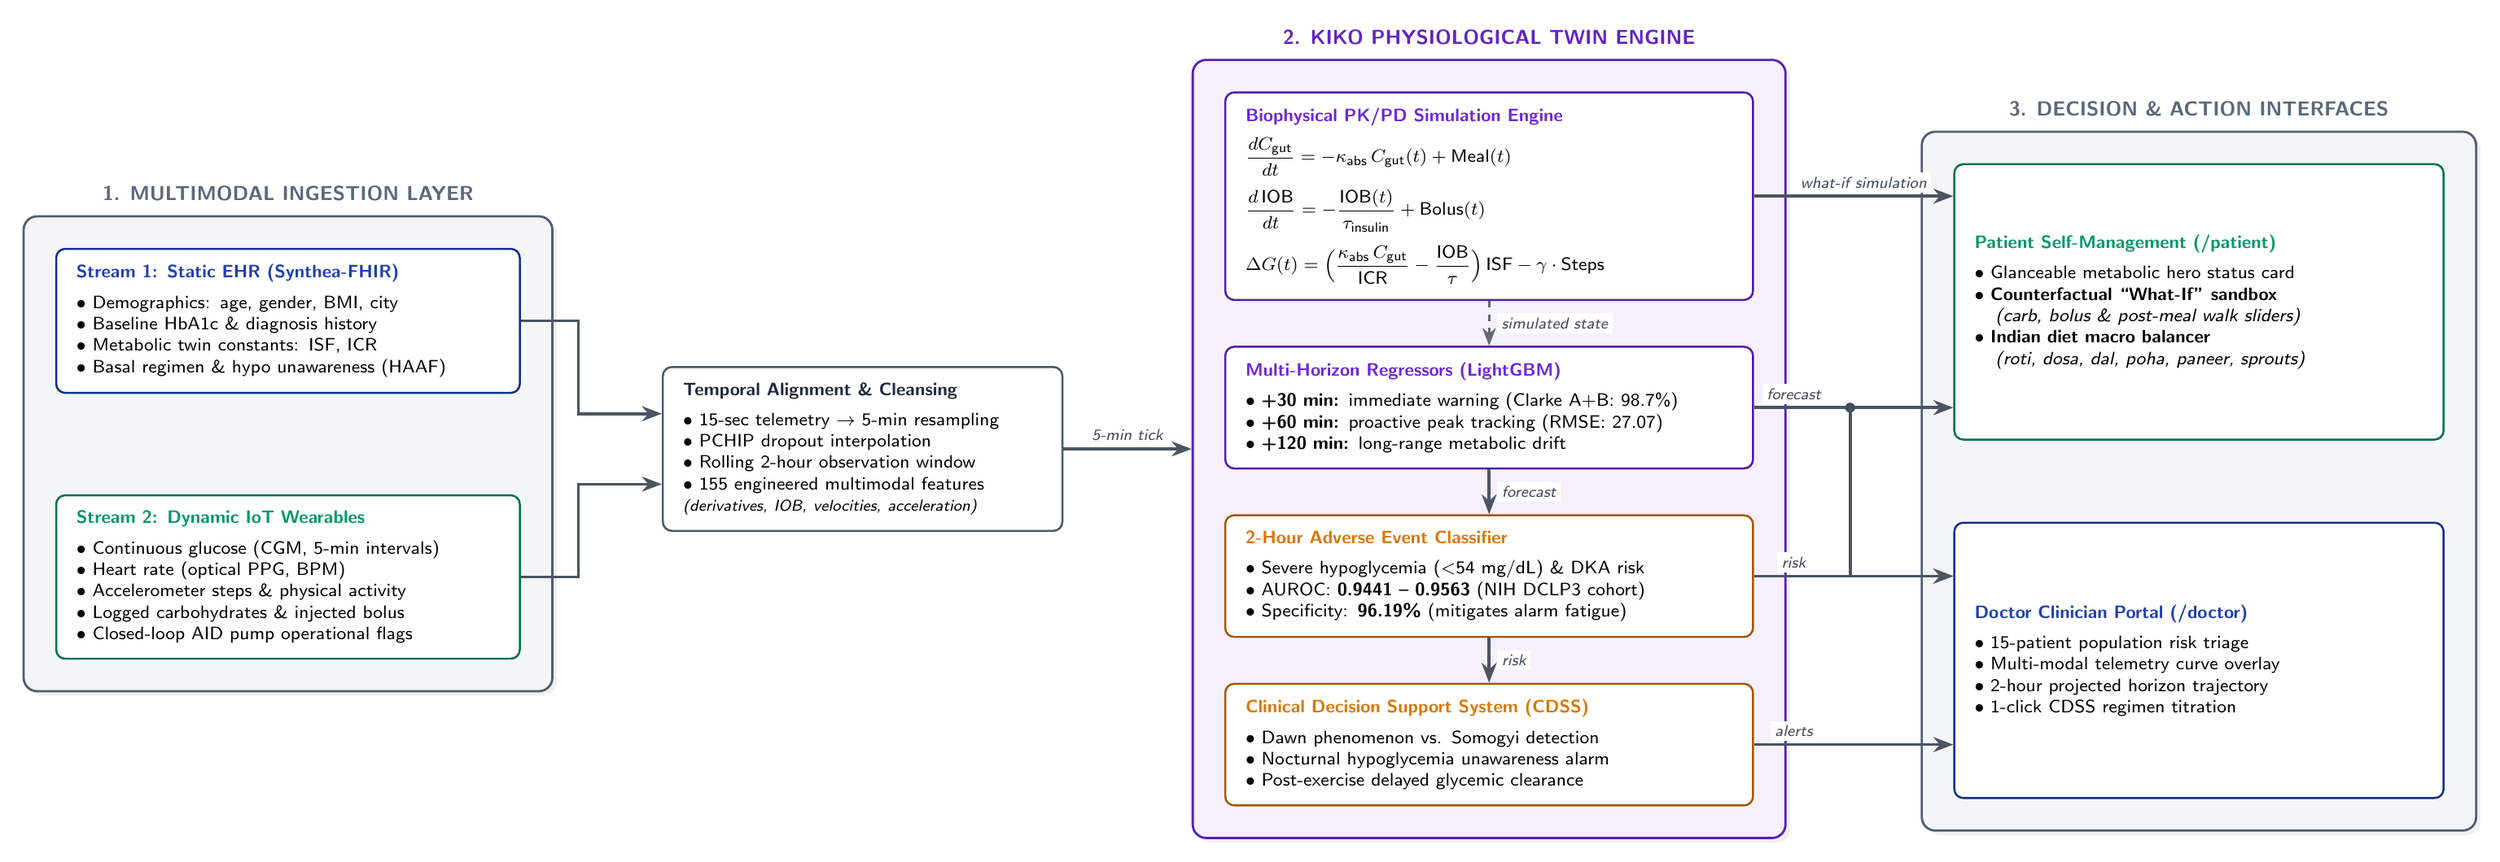
\begin{tikzpicture}[
    font=\sffamily,
    >=Stealth,
    box/.style={rectangle, rounded corners=6pt, draw=#1!80!black, line width=1pt,
        fill=#1!7, drop shadow={opacity=0.12, shadow xshift=2pt, shadow yshift=-2pt}},
    subbox/.style={rectangle, rounded corners=4pt, draw=#1!75!black, line width=0.9pt,
        fill=white, align=left, inner xsep=9pt, inner ysep=7pt, font=\sffamily\footnotesize},
    titlebox/.style={font=\sffamily\bfseries\small, text=#1!90!black},
    arrow/.style={->, line width=1.3pt, draw=darkslate!80},
    dashedarrow/.style={->, dashed, line width=1.1pt, draw=darkslate!70},
    lbl/.style={font=\sffamily\scriptsize\itshape, text=darkslate!85, fill=white, inner sep=2pt}
]

% ======================= 2. TWIN ENGINE (placed first, centre column) =======================
\node[subbox=corepurple, text width=7.6cm] (pkpd) {
    \textbf{\textcolor{corepurple}{Biophysical PK/PD Simulation Engine}}\\[4pt]
    $\dfrac{dC_{\text{gut}}}{dt} = -\kappa_{\text{abs}}\,C_{\text{gut}}(t) + \text{Meal}(t)$\\[5pt]
    $\dfrac{d\,\text{IOB}}{dt} = -\dfrac{\text{IOB}(t)}{\tau_{\text{insulin}}} + \text{Bolus}(t)$\\[5pt]
    $\Delta G(t) = \Big(\dfrac{\kappa_{\text{abs}}\,C_{\text{gut}}}{\text{ICR}} - \dfrac{\text{IOB}}{\tau}\Big)\,\text{ISF} - \gamma\cdot\text{Steps}$
};
\node[subbox=corepurple, text width=7.6cm, below=0.7cm of pkpd] (forecaster) {
    \textbf{\textcolor{corepurple}{Multi-Horizon Regressors (LightGBM)}}\\[4pt]
    $\bullet$ \textbf{+30 min:} immediate warning (Clarke A+B: 98.7\%)\\
    $\bullet$ \textbf{+60 min:} proactive peak tracking (RMSE: 27.07)\\
    $\bullet$ \textbf{+120 min:} long-range metabolic drift
};
\node[subbox=amberalert, text width=7.6cm, below=0.7cm of forecaster] (classifier) {
    \textbf{\textcolor{amberalert}{2-Hour Adverse Event Classifier}}\\[4pt]
    $\bullet$ Severe hypoglycemia ($<$54 mg/dL) \& DKA risk\\
    $\bullet$ AUROC: \textbf{0.9441 -- 0.9563} (NIH DCLP3 cohort)\\
    $\bullet$ Specificity: \textbf{96.19\%} (mitigates alarm fatigue)
};
\node[subbox=amberalert, text width=7.6cm, below=0.7cm of classifier] (cdss) {
    \textbf{\textcolor{amberalert}{Clinical Decision Support System (CDSS)}}\\[4pt]
    $\bullet$ Dawn phenomenon vs. Somogyi detection\\
    $\bullet$ Nocturnal hypoglycemia unawareness alarm\\
    $\bullet$ Post-exercise delayed glycemic clearance
};
\begin{scope}[on background layer]
    \node[box=corepurple, fit=(pkpd)(forecaster)(classifier)(cdss), inner sep=14pt,
        label={[titlebox=corepurple, above=3pt]north:\textbf{2. KIKO PHYSIOLOGICAL TWIN ENGINE}}] (engine) {};
\end{scope}
\draw[dashedarrow] (pkpd.south) -- node[lbl, right=3pt]{simulated state} (forecaster.north);
\draw[arrow] (forecaster.south) -- node[lbl, right=3pt]{forecast} (classifier.north);
\draw[arrow] (classifier.south) -- node[lbl, right=3pt]{risk} (cdss.north);

% ======================= PREPROCESSING (left of engine, vertically centred) =======================
\node[subbox=slateborder, text width=5.6cm, left=2.0cm of engine] (pre) {
    \textbf{\textcolor{darkslate}{Temporal Alignment \& Cleansing}}\\[4pt]
    $\bullet$ 15-sec telemetry $\rightarrow$ 5-min resampling\\
    $\bullet$ PCHIP dropout interpolation\\
    $\bullet$ Rolling 2-hour observation window\\
    $\bullet$ 155 engineered multimodal features\\
    \textit{\scriptsize(derivatives, IOB, velocities, acceleration)}
};
\draw[arrow] (pre.east) -- node[lbl, above=1pt]{5-min tick} (engine.west |- pre.east);

% ======================= 1. INGESTION (left of preprocessing) =======================
\node[subbox=ehrblue, text width=6.6cm, anchor=east] (ehr) at ($(pre.west)+(-2.2cm, 2.0cm)$) {
    \textbf{\textcolor{ehrblue}{Stream 1: Static EHR (Synthea-FHIR)}}\\[4pt]
    $\bullet$ Demographics: age, gender, BMI, city\\
    $\bullet$ Baseline HbA1c \& diagnosis history\\
    $\bullet$ Metabolic twin constants: ISF, ICR\\
    $\bullet$ Basal regimen \& hypo unawareness (HAAF)
};
\node[subbox=iotgreen, text width=6.6cm, anchor=east] (wear) at ($(pre.west)+(-2.2cm, -2.0cm)$) {
    \textbf{\textcolor{iotgreen}{Stream 2: Dynamic IoT Wearables}}\\[4pt]
    $\bullet$ Continuous glucose (CGM, 5-min intervals)\\
    $\bullet$ Heart rate (optical PPG, BPM)\\
    $\bullet$ Accelerometer steps \& physical activity\\
    $\bullet$ Logged carbohydrates \& injected bolus\\
    $\bullet$ Closed-loop AID pump operational flags
};
\begin{scope}[on background layer]
    \node[box=slateborder, fit=(ehr)(wear), inner sep=14pt,
        label={[titlebox=slateborder, above=3pt]north:\textbf{1. MULTIMODAL INGESTION LAYER}}] (ingest) {};
\end{scope}
\draw[arrow] (ehr.east) -- ++(0.9,0) |- ([yshift=0.55cm]pre.west);
\draw[arrow] (wear.east) -- ++(0.9,0) |- ([yshift=-0.55cm]pre.west);

% ======================= 3. INTERFACES (right of engine) =======================
\node[subbox=iotgreen, text width=7.0cm, minimum height=4.3cm, anchor=west]
    (patient) at ($(engine.east |- {$(pkpd.east)!0.5!(forecaster.east)$})+(2.6cm,0)$) {
    \textbf{\textcolor{iotgreen}{Patient Self-Management (/patient)}}\\[4pt]
    $\bullet$ Glanceable metabolic hero status card\\
    $\bullet$ \textbf{Counterfactual ``What-If'' sandbox}\\
    \hspace*{1.1em}\textit{(carb, bolus \& post-meal walk sliders)}\\
    $\bullet$ \textbf{Indian diet macro balancer}\\
    \hspace*{1.1em}\textit{(roti, dosa, dal, poha, paneer, sprouts)}
};
\node[subbox=ehrblue, text width=7.0cm, minimum height=4.3cm, anchor=west]
    (doctor) at ($(engine.east |- {$(classifier.east)!0.5!(cdss.east)$})+(2.6cm,0)$) {
    \textbf{\textcolor{ehrblue}{Doctor Clinician Portal (/doctor)}}\\[4pt]
    $\bullet$ 15-patient population risk triage\\
    $\bullet$ Multi-modal telemetry curve overlay\\
    $\bullet$ 2-hour projected horizon trajectory\\
    $\bullet$ 1-click CDSS regimen titration
};
\begin{scope}[on background layer]
    \node[box=slateborder, fit=(patient)(doctor), inner sep=14pt,
        label={[titlebox=slateborder, above=3pt]north:\textbf{3. DECISION \& ACTION INTERFACES}}] (ui) {};
\end{scope}

% ======================= Engine -> interfaces (one clean channel per output) =======================
\draw[arrow] (pkpd.east) -- node[lbl, above=1pt, pos=0.55]{what-if simulation} (pkpd.east -| patient.west);
\coordinate (J) at ($(forecaster.east)+(1.5cm,0)$);
\draw[arrow] (forecaster.east) -- node[lbl, above=1pt, pos=0.2]{forecast} (forecaster.east -| patient.west);
\fill[darkslate!85] (J) circle (2.2pt);
\draw[arrow] (J) -- (J |- classifier.east) -- (classifier.east -| doctor.west);
\draw[arrow] (classifier.east) -- node[lbl, above=1pt, pos=0.2]{risk} (classifier.east -| doctor.west);
\draw[arrow] (cdss.east) -- node[lbl, above=1pt, pos=0.2]{alerts} (cdss.east -| doctor.west);

\end{tikzpicture}
\end{document}
